

\tikzset{every picture/.style={line width=0.75pt}} %set default line width to 0.75pt        

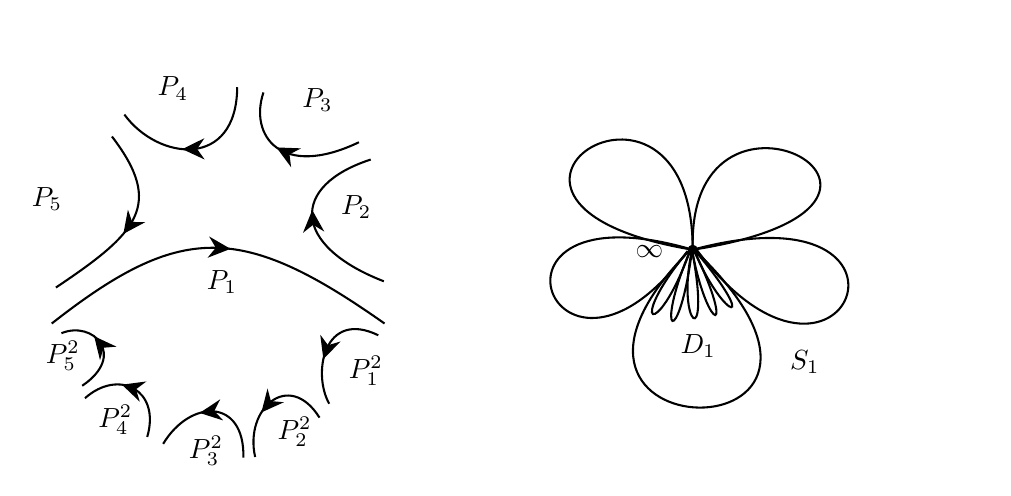
\begin{tikzpicture}[x=0.75pt,y=0.75pt,yscale=-1,xscale=1]
%uncomment if require: \path (0,300); %set diagram left start at 0, and has height of 300

%Curve Lines [id:da8105529734511654] 
\draw    (108,57.17) .. controls (124.33,79.5) and (162.07,83.64) .. (162.35,44) ;
\draw [shift={(135.91,73.82)}, rotate = 359.3] [fill={rgb, 255:red, 0; green, 0; blue, 0 }  ][line width=0.08]  [draw opacity=0] (10.72,-5.15) -- (0,0) -- (10.72,5.15) -- (7.12,0) -- cycle    ;
%Curve Lines [id:da5656492723103168] 
\draw    (226.67,78.83) .. controls (187.67,91.5) and (188.33,120.17) .. (233,137.5) ;
\draw [shift={(198.51,103.16)}, rotate = 86.49] [fill={rgb, 255:red, 0; green, 0; blue, 0 }  ][line width=0.08]  [draw opacity=0] (10.72,-5.15) -- (0,0) -- (10.72,5.15) -- (7.12,0) -- cycle    ;
%Curve Lines [id:da13626418538311813] 
\draw    (233.33,157.83) .. controls (164.33,109.17) and (135,109.17) .. (73,157.83) ;
\draw [shift={(159.13,121.86)}, rotate = 184.37] [fill={rgb, 255:red, 0; green, 0; blue, 0 }  ][line width=0.08]  [draw opacity=0] (10.72,-5.15) -- (0,0) -- (10.72,5.15) -- (7.12,0) -- cycle    ;
%Curve Lines [id:da4850842944262794] 
\draw    (126.67,215.83) .. controls (139.67,194.17) and (166,193.5) .. (165.33,222.5) ;
\draw [shift={(144.27,200.92)}, rotate = 352.09] [fill={rgb, 255:red, 0; green, 0; blue, 0 }  ][line width=0.08]  [draw opacity=0] (10.72,-5.15) -- (0,0) -- (10.72,5.15) -- (7.12,0) -- cycle    ;
%Curve Lines [id:da6830177286463675] 
\draw    (206.67,196.5) .. controls (198.33,181.5) and (204.33,150.83) .. (230.33,163.5) ;
\draw [shift={(203.85,175.03)}, rotate = 288.5] [fill={rgb, 255:red, 0; green, 0; blue, 0 }  ][line width=0.08]  [draw opacity=0] (10.72,-5.15) -- (0,0) -- (10.72,5.15) -- (7.12,0) -- cycle    ;
%Curve Lines [id:da8979306236335514] 
\draw    (171,222.17) .. controls (165.67,198.83) and (187.33,179.83) .. (202,203.17) ;
\draw [shift={(174.01,200.66)}, rotate = 310] [fill={rgb, 255:red, 0; green, 0; blue, 0 }  ][line width=0.08]  [draw opacity=0] (10.72,-5.15) -- (0,0) -- (10.72,5.15) -- (7.12,0) -- cycle    ;
%Shape: Circle [id:dp28811964079698127] 
\draw  [fill={rgb, 255:red, 0; green, 0; blue, 0 }  ,fill opacity=1 ] (379.9,122.3) .. controls (379.9,121.25) and (380.75,120.4) .. (381.8,120.4) .. controls (382.85,120.4) and (383.7,121.25) .. (383.7,122.3) .. controls (383.7,123.35) and (382.85,124.2) .. (381.8,124.2) .. controls (380.75,124.2) and (379.9,123.35) .. (379.9,122.3) -- cycle ;
%Curve Lines [id:da9630686419392767] 
\draw    (382.79,122.56) .. controls (490.56,225) and (281,222.33) .. (380.79,122.19) ;
%Curve Lines [id:da6952983011098728] 
\draw    (381.8,122.3) .. controls (520.87,100.6) and (380.47,25) .. (381.8,120.4) ;
%Curve Lines [id:da414714992696418] 
\draw    (381.8,120.4) .. controls (380.07,15.8) and (249.27,100.2) .. (381.8,122.3) ;
%Curve Lines [id:da63508389820832] 
\draw    (380.29,123.44) .. controls (364.42,167.06) and (349.66,159.26) .. (378.79,123.81) ;
%Curve Lines [id:da22495593911989342] 
\draw    (381.8,124.2) .. controls (389.29,162.69) and (402.79,164.81) .. (382.79,123.31) ;
%Curve Lines [id:da16912708964122225] 
\draw    (382.79,123.31) .. controls (397.36,157.62) and (414.9,160.38) .. (382.79,122.56) ;
%Curve Lines [id:da7915056796916238] 
\draw    (175,46.5) .. controls (168,67.17) and (183.33,88.5) .. (221,70.5) ;
\draw [shift={(181.25,73)}, rotate = 27.81] [fill={rgb, 255:red, 0; green, 0; blue, 0 }  ][line width=0.08]  [draw opacity=0] (10.72,-5.15) -- (0,0) -- (10.72,5.15) -- (7.12,0) -- cycle    ;
%Curve Lines [id:da06174169363528992] 
\draw    (102,67.73) .. controls (127.33,100.83) and (114.33,114.17) .. (75,140.5) ;
\draw [shift={(107.51,114.63)}, rotate = 306.28] [fill={rgb, 255:red, 0; green, 0; blue, 0 }  ][line width=0.08]  [draw opacity=0] (10.72,-5.15) -- (0,0) -- (10.72,5.15) -- (7.12,0) -- cycle    ;
%Curve Lines [id:da6193229855841036] 
\draw    (89,193.83) .. controls (105,179.5) and (125.67,189.5) .. (119,212.5) ;
\draw [shift={(106.83,187.31)}, rotate = 18.1] [fill={rgb, 255:red, 0; green, 0; blue, 0 }  ][line width=0.08]  [draw opacity=0] (10.72,-5.15) -- (0,0) -- (10.72,5.15) -- (7.12,0) -- cycle    ;
%Curve Lines [id:da06319156006210047] 
\draw    (77.67,162.5) .. controls (93,156.17) and (109.33,173.17) .. (87.67,187.83) ;
\draw [shift={(93.44,163.98)}, rotate = 50.62] [fill={rgb, 255:red, 0; green, 0; blue, 0 }  ][line width=0.08]  [draw opacity=0] (10.72,-5.15) -- (0,0) -- (10.72,5.15) -- (7.12,0) -- cycle    ;
%Curve Lines [id:da600082967290146] 
\draw    (383.7,122.3) .. controls (455.25,217.04) and (504.87,89) .. (381.8,122.3) ;
%Curve Lines [id:da0010692790397923702] 
\draw    (379.29,122.94) .. controls (315.27,210.2) and (268.87,89) .. (381.8,122.3) ;
%Curve Lines [id:da9686102352343344] 
\draw    (381.17,124.06) .. controls (373.92,158.69) and (390.67,172.31) .. (381.8,124.2) ;
%Curve Lines [id:da07465915682499946] 
\draw    (380.29,123.44) .. controls (363.04,164.31) and (375.17,171.19) .. (381.42,122.94) ;

% Text Node
\draw (146.29,130.84) node [anchor=north west][inner sep=0.75pt]    {$P_{1}$};
% Text Node
\draw (210.95,94.51) node [anchor=north west][inner sep=0.75pt]    {$P_{2}$};
% Text Node
\draw (192.24,42.92) node [anchor=north west][inner sep=0.75pt]    {$P_{3}$};
% Text Node
\draw (214.62,171.84) node [anchor=north west][inner sep=0.75pt]    {$P_{1}^{2}$};
% Text Node
\draw (180.29,201.51) node [anchor=north west][inner sep=0.75pt]    {$P_{2}^{2}$};
% Text Node
\draw (137.62,210.51) node [anchor=north west][inner sep=0.75pt]    {$P_{3}^{2}$};
% Text Node
\draw (352.81,118.66) node [anchor=north west][inner sep=0.75pt]    {$\infty $};
% Text Node
\draw (374.46,161.54) node [anchor=north west][inner sep=0.75pt]    {$D_{1}$};
% Text Node
\draw (427.23,169.33) node [anchor=north west][inner sep=0.75pt]    {$S_{1}$};
% Text Node
\draw (122.57,37.59) node [anchor=north west][inner sep=0.75pt]    {$P_{4}$};
% Text Node
\draw (61.9,90.92) node [anchor=north west][inner sep=0.75pt]    {$P_{5}$};
% Text Node
\draw (93.95,195.51) node [anchor=north west][inner sep=0.75pt]    {$P_{4}^{2}$};
% Text Node
\draw (68.62,164.84) node [anchor=north west][inner sep=0.75pt]    {$P_{5}^{2}$};


\end{tikzpicture}